In this section we describe our model and compare it to a number of different baseline models. We implement our model as well as the baselines in Python 3.7 using NumPy, Pandas, Scikit-learn and PyTorch. We split the training data into training and test datasets randomly while ensuring that the distributions of human/bot labels in both datasets represent the overall distribution accurately. 
We evaluate the model against Gaussian Naïve Bayes (GNB), Quadratic Discriminant Analysis (QDA), a Support Vector Machine (SVM), a $k$-Nearest Neighbors (KNN) and a Random Forest (RF) model. For these baseline models we use the following features:
\begin{align*}
    X_{base} = \{ & \texttt{default\_profile}, \texttt{profile\_image}, \texttt{favourites\_count}, \\
    & \texttt{followers}, \texttt{following}, \texttt{listed\_count}, \texttt{statuses\_count}, \\
    & \texttt{account\_age}, \texttt{reputation} \}
\end{align*}

We evaluated linear, polynomial and RBF kernels for the SVM model and found the model to perform best with the RBF kernel. The RF model is trained using 100 trees, and splits are performed according to the Gini coefficient. GNB and QDA models are trained using the standard settings in Scikit-learn. 

The neural network classifier is a fully-connected feedforward neural network. After much experimentation we chose to use 3 hidden layers with $(500, 200, 100)$ neurons respectively, using batch normalization and dropout with $p=0.5$. The model is trained using Adam and a learning rate of $\theta = 1e-3$ for 750 epochs. We find that the model achieves better performance and generalizes better when we remove outliers that deviate from the mean by more than three standard deviations from the training dataset.

We experimented with different sets of features and found a set of neighborhood features (NF) and graph features (GF) described in section \ref{sec:approach} that performs best along with the baseline features. We also found that removing some of the original features along with adding the  NF and GF improved the performance of our classification model. The set of features used in our classifier are:
\begin{alignat*}{2}
    & X_{NF} = \{ && \texttt{favourites\_count}, \texttt{statuses\_count}, \texttt{indegree\_successors}, \\
    & && \texttt{outdegree\_predecessors}, \texttt{favorites\_predecessors}, \\
    & && \texttt{favorites\_successors}, \texttt{status\_predecessors}, \\
    & && \texttt{age\_predecessors}, \texttt{account\_age}, \\
    & && \texttt{following}, \texttt{listed\_count} \} \\
    \\
    & X_{GF} = && \{ \texttt{ego\_density}, \texttt{ego\_reciprocity} \}
\end{alignat*}

\begin{figure}
    \centering
    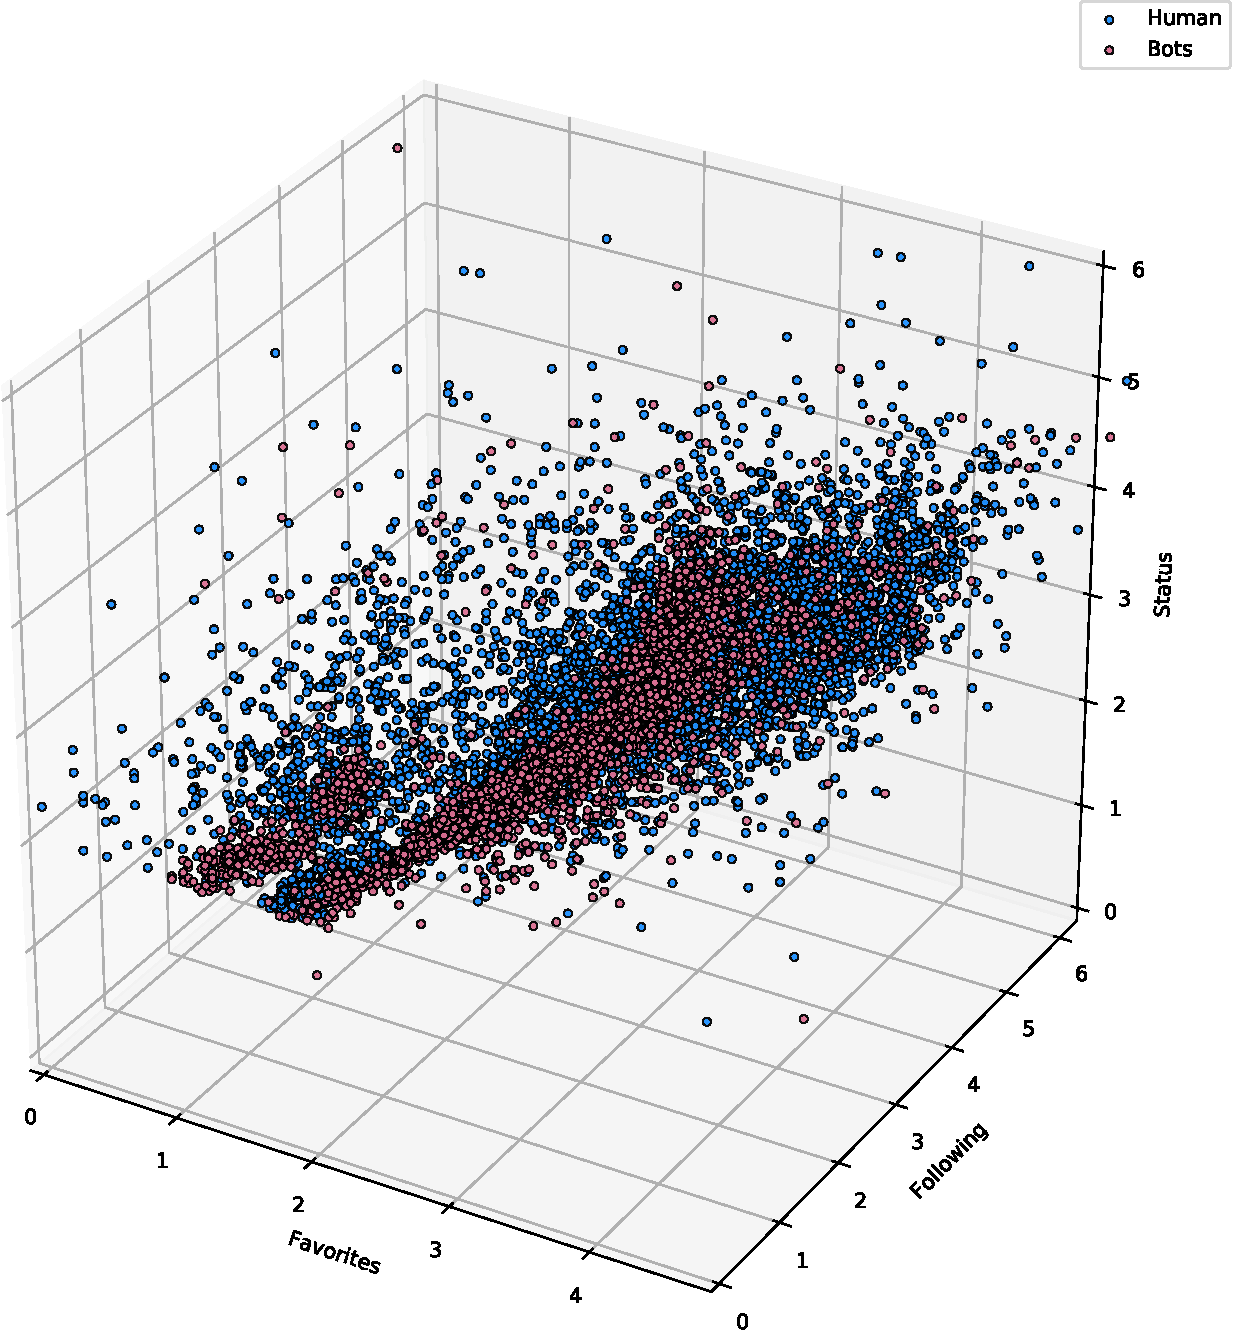
\includegraphics[width=0.8\textwidth]{paper/FIG/3dvis_base-crop.pdf}
    \caption{We can clearly see the different distributions of human }
    \label{fig:my_label}
\end{figure}

\noindent It is interesting to note that actually only a certain, very few features are necessary to effectively separate bots and humans in multi-dimensional space. We find that the number of a user's favourites, followers and statuses actually suffice to identify very clear differences in the distribution of human and bot accounts (Figure \ref{fig:3dvis}). Indeed, a RF classifier is able to achieve and F1 score of 0.8781 and AUC of 0.8705 using only those three features.

Our model outperforms the baseline models on the \textsc{Cresci-2018} dataset (table~\ref{tab:results}). We notice that both the GNB and QDA model are not very good at identifying bot accounts on this dataset accurately and have a very high false positive rate. The SVM model is slightly better and achieves an F1 score of 0.79. Interestingly, KNN is surprisingly effective on this dataset and only slightly less effective than the RF and NN models. Both RF and NN turn out to be very effective and achieve the highest scores. Due to this we chose to focus on RF and NN for our model. By using the proposed NF features we see an overall improvement both for the RF and NN models.

\begin{table}[t]
\centering
\begin{tabular}{@{}lccccc@{}}
\toprule
\textbf{Model} & \textbf{Acc} & \textbf{TPR} & \textbf{FPR} & \textbf{F1 score} & \textbf{AUC} \\ \midrule
GNB             & 0.6399 & 0.9622 & 0.7313 & 0.741  & 0.6154 \\
QDA             & 0.6751 & 0.8937 & 0.5768 & 0.7465 & 0.6584 \\
SVM             & 0.7797 & 0.7746 & 0.2145 & 0.7901 & 0.7801 \\
KNN             & 0.8496 & 0.8752 & 0.18   & 0.8617 & 0.8476 \\
Random forest   & 0.8675 & 0.8745 & 0.1405 & 0.876  & 0.867 \\
NN              & 0.50   & 0.50   & 0.50   & 0.50   & 0.50 \\ \midrule
NN + NF (ours)  & 0.8683 & 0.8816 & 0.1471 & 0.8775 & 0.8673 \\
NN + NF + GF (ours) & \textbf{0.90} & \textbf{0.01} & \textbf{0.90} & \textbf{0.90} & \textbf{0.90} \\
RF + NF + GF (ours) & 0.8771 & 0.8873 & 0.1346 & 0.8854 & 0.8763 \\
\bottomrule
\end{tabular}
\caption{Placeholder evaluation results}
\label{tab:results}
\end{table}